% !TEX root = ../../main.tex

\section{Compliance in porous crystals}

\subsection{Examining the assumption of an inert adsorbent}

Adsorption induced changes in porous media have been known
to occur for over 90 years~\cite{mcbainNatureInfluenceHumidity1927},
with both clays, coals and polymers undergoing swelling during gas
or vapour uptake~\cite{gorAdsorptioninducedDeformationNanoporous2017}.
However, the effect upon the macroscopic properties of the material is 
often negligibly small and of little consequence to industrial adsorption
processes. Studies of this aspect of porous adsorbents have therefore
been scarce in the large part of the 20\textsuperscript{th} century,
likewise influenced by lack of sufficiently accurate methods for 
characterising and modelling such occurrences.

In recent years, the advent of reference materials, 
highly sensitive methods such as synchrotron-grade light sources and
\textit{in silico} computational techniques such as DFT has put at
our disposal the tools required to study these transformations. 
Together with the discovery of their role in natural and industrial 
processes e.g.\ the swelling of shale during natural gas extraction,
maturation of concrete and the perspectives afforded by novel porous
materials, these factors have generated much scientific interest
in material compliance. As an example, the attractive option
of combined carbon capture and methane recovery implemented 
through pumping of carbon dioxide into reservoirs is prohibited
by swelling-induced loss of porosity and well 
blocking~\cite{gorAdsorptioninducedDeformationNanoporous2017}. 

In-depth studies~\cite{beringAlterationZeoliteGranule1977} 
have revealed that most porous materials posses some small
degree of compliance, with \textit{in-situ} dilatometry going so far as to 
obtain pore size distributions from accurate volume
changes~\cite{reichenauerExtractingPoreSize2001}. Most flexible 
processes can be likened to continuous order transitions. It is, however,
the discovery of large scale flexibility in MOFs such as 
MIL-53 and linker-controlled gate opening like in ZIF-8, 
where the transformation between the different framework 
states occurs suddenly at precise points in the loading curve,
which has shown that compliance may also take the form of 
a first-order transition. Such types of transformations are
desirable~\cite{kitagawaFunctionalPorousCoordination2004} due to 
their highly specific response. The possible dependence 
of flexibility on other stimuli, such as light, mechanical pressure,
temperature or magnetic fields may allow for precise tuning of 
structural changes. As such, it is reasonable to state that
the mobility of the solid phase can no longer be ignored.

\subsection{Flexibility in metal organic frameworks}

Since the highlight of compliance in porous coordination polymers 
in the report of~\citet{kitagawaFunctionalPorousCoordination2004},
much progress has been made in the synthesis and understanding
of this phenomenon. An exhaustive review of MOF flexibility is 
outside the scope of this thesis, with the field progressing 
rapidly enough to generate a wealth of critical
literature~\cite{schneemannFlexibleMetalOrganic2014, %
fereyHybridPorousSolids2008, liMetalOrganicFrameworks2012, %
haldarInterpenetrationCoordinationPolymers2015, %
stassenUpdatedRoadmapIntegration2017, %
vanduyfhuysThermodynamicInsightStimuliresponsive2018, %
murdockApproachesSynthesizingBreathing2014}.
Some of the known types of structural flexibility encountered in MOFs
will be briefly discussed, with a summary available in 
\autoref{dut:fgr:flex-types}. 

\begin{figure}[htb]
    \centering
    
    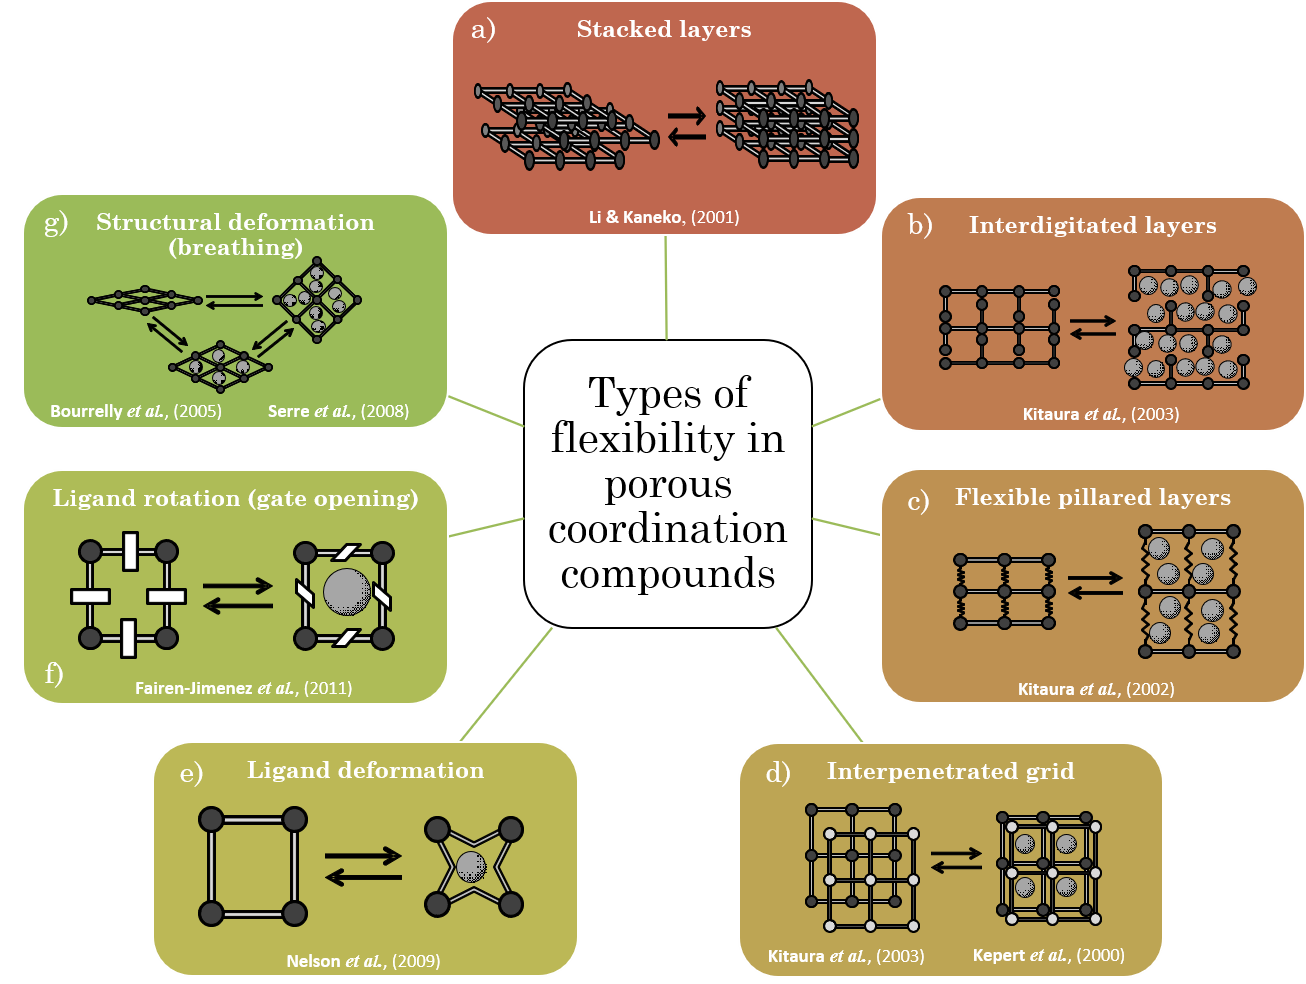
\includegraphics[width=\textwidth]{flexibility-types}%
    \caption{A (non-exhaustive) visual summary of the types of
    flexibility documented in MOFs, as detailed in 
    (a)~\citet{liHydrogenBondregulatedMicroporous2001}
    (b)~\citet{kitauraPorousCoordinationPolymerCrystals2003}
    (c)~\citet{kitauraPillaredLayerCoordinationPolymer2002}
    (d)~\citet{kepertVersatileFamilyInterconvertible2000,%
    kitauraPorousCoordinationPolymerCrystals2003}
    (e)~\citet{nelsonSupercriticalProcessingRoute2009}
    (f)~\citet{fairen-jimenezOpeningGateFramework2011}
    (g)~\citet{bourrellyDifferentAdsorptionBehaviors2005, %
    serreExplanationVeryLarge2007}}%
    \label{dut:fgr:flex-types}
    
\end{figure}

Since MOFs, like clays and graphite, can form discrete 
two-dimensional sheets, bound together by weak Van-der-Waals,
\( \pi-\pi \) interactions or hydrogen bonds,
adsorbed molecules may force these layers apart by 
intercalation. The concept is taken further in the 
pillared layer approach, where the sheets are connected 
by tertiary linkers instead of weak attractions. With the 
judicious choice of linker, these can act as springs, allowing
pore expansion while maintaining structural integrity.

As briefly mentioned in \autoref{def}, a large void 
space in the unit cells allows secondary networks 
to grow throughout the MOF, effectively creating an 
intercalated structure~\cite{kepertVersatileFamilyInterconvertible2000,%
kitauraPorousCoordinationPolymerCrystals2003}. 
These secondary grids are independent
of the primary framework and are displaced upon guest 
adsorption~\cite{majiFlexibleInterpenetratingCoordination2007}. 
This internal translation may also be associated 
with a tilting of the 
linker~\cite{sakataShapeMemoryNanoporesInduced2013},
combining intercalation with structural-deformation type 
flexibility.

The origin of flexibility may be purely due to the linker 
itself. Organic bonds are inherently labile, as seen in 
polymer chains, since unsaturated connections in the linker may
bend if the strain on the organic strut overcomes its tensile 
strength. Increasing the linker length often induces this 
type of flexibility, for example in the IRMOF isoreticular series
of materials~\cite{nelsonSupercriticalProcessingRoute2009}.
Even an unsaturated bond may be induced by a photon with a 
suitable energy to undergo an analogue of a \textit{cis-trans}
transition. The deformation may also lead to expansion and 
therefore of framework swelling,
as encountered in MIL-88 and its
derivatives~\cite{maIronBasedMetalOrganic2013}.

MOFs can also have structural flexibility which does not
require any volume changes in the unit cell. The rotation of linkers
can act as gating for different guests, allowing entry of probes
larger than the window size would suggest or preferential adsorption
of a gas which has the right property to act as a ``key'' from 
a mixture~\cite{seoPillaredLayerCoordinationPolymer2009}. 
The former effect is common in zeolitic imidazole frameworks 
(ZIFs)~\cite{fairen-jimenezOpeningGateFramework2011}.

The discovery of the so-called ``breathing'' type of structural
deformation~\cite{loiseauRationaleLargeBreathing2004, %
bourrellyDifferentAdsorptionBehaviors2005, %
    serreExplanationVeryLarge2007} in the MIL-53 and MIL-47 family of
materials has revealed step-like transformations in its unit cell
size and metastable intermediaries with an open pore (\textit{op}), 
closed pore (\textit{cp}) and narrow/intermediate states (\textit{np}/
\textit{ip}).
No other family of flexible MOFs has, to date, generated
more scientific interest. This is likely due to the relative 
stability of the material, combined with its ability to undergo massive 
and reversible structural deflections, while retaining its 
crystalinity. The relatively simple structure and large capability 
for functionalisation, either through ligand modification or exchange
of the metal node (with variants of MIL-53 synthesised for Cr, Fe, Al,
Sc, Ga or In), allowed for its use as an archetypal material 
for the study of flexible behaviour. More recently, similar 
materials, like DUT-8(M) (M=Ni, Co, Cu, Zn) which allow the the 
impact of the 
metal~\cite{kleinStructuralFlexibilityIntrinsic2012} on
compliance to be evidenced have emerged.

\subsection{Describing and inducing MOF compliance}

The mechanistic phenomena during adsorption can be 
seen as an overlap~\cite{gorAdsorptionInducedDeformationMesoporous2010}
of several competing effects: a sub-monolayer
contraction~\cite{daceyVolumeChangesSaran1971} resulting
from micropore bridging or surface stresses, followed by a monotonic 
expansion with the gradual decrease of the solid-fluid interface energy
also known as the Bangham 
effect~\cite{banghamExpansionCharcoalAccompanying1928}. 
Such behaviour is highly dependent of pore size, geometry and anisotropy,
with condensation in macropores a further complex source of 
strain~\cite{dolinoAdsorptionStrainsPorous1996, %
ambergSTUDYADSORPTIONHYSTERESIS1952, %
guntherNovelInsightsNanopore2008}. The degree of adsorption induced
changes in a framework is generally a function of its porosity, 
with very high 
surface area materials such as aerogels capable of undergoing up 
to 30\% deformation~\cite{reichenauerNitrogenSorptionAerogels2001}.
In MOFs, the adsorption stresses are no different than in other 
materials. However, the ability of the porous network to undergo
displacements is much higher, since its rigidity is in 
between that of ``hard'' adsorbents such as zeolites/silica and 
purely organic polymers (although porous covalent frameworks can
also achieve self-support and porosity).

Finding a suitable model that would predict both the adsorption
induced stress and the resulting structural changes from strain
has so far remained a challenge. A thermodynamic-based method which
has been successfully applied to breathing MOFs is that 
of~\citet{neimarkStressBasedModelBreathing2010}. This model assumes
that the deformation strain is fully determined due to surface stress,
calculated from the grand thermodynamical of a rigid analogue of
the pore. It has been used to explain the existence 
domains of MIL-53(Al)~\cite{boutinBehaviorFlexibleMIL532010}, in 
conjunction with an osmotic thermodynamic description of 
the framework itself~\cite{coudertThermodynamicsGuestInducedStructural2008}.
For mesoporous materials, the stress-strain model has been extended 
by~\citet{gorAdsorptionInducedDeformationMesoporous2010} through
the Derjaguin–Broekhoff–de Boer (DBdB) 
theory~\cite{broekhoffStudiesPoreSystems1967} and applied to
predict the resulting strain in mesoporous silica.
Nevertheless a complete theory of adsorption-deformation 
which can fully predict the changes in the measured enthalpy of 
adsorption and the mechanistic behaviour of MOFs has remained elusive.

The most promising characteristics of flexible MOFs are the ability
to control the compliance through external means which are 
detached from guest loading, which would dramatically expand
their potential applications. 
Pure mechanical pressure on a flexible material 
is often enough to induce transitions. First observed on 
ZIFs, through pressure induced phase 
change~\cite{chapmanTrappingGuestsNanoporous2011, % 
tanMechanicalPropertiesHybrid2011} and 
latter applied to breathing MOFs using
mercury porosimetry~\cite{beurroiesUsingPressureProvoke2010, %
yotLargeBreathingMOF2012}, it 
shows a direct relationship between the bulk modulus of 
a MOF and its flexible behaviour.
Entropic control through temperature-induced switching has been
shown to be possible in MIL-53 
by~\citet{liuReversibleStructuralTransition2008}, explained 
as a change in the range of metastability of its 
pore forms~\cite{boutinBehaviorFlexibleMIL532010}. 
More precise external control may be possible if molecules which
have the ability to switch their state when exposed to suitable
wavelengths are used as linkers. In this case light irradiation 
may be used to force the 
transition~\cite{lyndonDynamicPhotoSwitchingMetalOrganic2013}.
Magnetic field dependent switching can also be theorised, although
has not been so far encountered.
One of the least understood factors that changes the flexible
behaviour of porous crystals is the effect of particle size.
It is clear that the thermodynamical potential of the crystal surface
has a a profound influence on its compliance, as shown on 
the large shift of the gate-opening pressure of 
ZIF-8~\cite{zhangCrystalSizeDependentStructuralTransitions2014}.
However, a rigorous model of the contribution of the surface 
on breathing has yet to be developed in our knowledge.
Finally, the presence of structural defects likely impacts 
the framework flexibility, as highlighted 
by~\citet{bennettInterplayDefectsDisorder2016} in a 
recent article, although currently few studies have focused
on this subject.

\subsection{Consequences and applications of flexible MOFs}

The study of flexible MOFs is motivated from both a desire 
for fundamental understanding of compliance and from the potential
applications of such systems. The use of soft porous crystals
in sensing and gas storage and separation is evident, although 
applications in catalysis, electrochemistry and drug delivery 
have also been alluded to by recent studies.

The usefulness of adsorption induced flexibility for sensors or
actuators has been been recognised, initially by nature itself,
with humidity induced swelling acting to open pine 
cones~\cite{dawsonHowPineCones1997}.
More recently, similar sensing devices based on adsorption strain 
in mesoporous silica have been 
developed such as a flexing silica-polymer 
membrane~\cite{boudotConvertingWaterAdsorption2016} or 
deformation of a nano sized 
cantilever~\cite{ganserCantileverBendingBased2016} 
which show promise for use in micromechanical systems. 

From a gas storage and separation point of view, changes in the
adsorbent structure may yield crucial process improvements. 
Pressure swing adsorption (PSA) is heavily
dependent on the working capacity of the adsorbent used, or the
difference between loading at the operation pressure and at the 
regeneration pressure. In this case, an S-shaped isotherm, with 
the vertical part of the slope in the aforementioned pressure 
range would lead to high process efficiency gains by eliminating material
``dead volume adsorbed''~\cite{schneemannFlexibleMetalOrganic2014}. 
In a temperature swing process (TSA), where 
the regeneration is performed through heating of the adsorbent 
bed, the key parameter is the integral enthalpy of adsorption, a measure 
of the energy requirements for the process. As a part of the chemical 
potential of the adsorbed phase is used by the mechanical contraction
of the material, flexible adsorbents have the advantage of
intrinsic thermal management, reducing the energy 
cost~\cite{masonMethaneStorageFlexible2015}.
Both effects are equally applicable to the storage of pure 
gasses, increasing the storage capacity and minimizing the energetic
requirement of recovery. Entrapment of guest molecules inside 
a gated pore might lend itself to temperature controlled storage and 
release of gasses~\cite{bunzenAchievingLargeVolumetric2018}, or
``sealing'' of a target gas inside the structure once adsorption
has taken place.
It is also possible that by using external mechanical pressure to
control flexibility, the adsorption behaviour of porous materials
may be tuned, as suggested by the work 
of~\citet{chanutUsingExternalFactors2016} on MIL-53. 

Catalytic applications of flexible MOFs could be envisaged where 
the switching behaviour can bring into contact active sites or 
hold reactants in place until complete reaction has taken place.
A recent study by~\citet{soutoBreathingDependentRedoxActivity2018},
has shown that the redox potential of the sulphur bond in a 
tetrathiafulvalene breathing MOF is dependent on its dihedral 
angle in different pore states. This raises the possibility of 
tunability of the oxidation potential of flexible framework.
Finally flexible MOFs constructed of biocompatible materials 
could be used as drug delivery 
methods~\cite{mckinlayNitricOxideAdsorption2013, %
horcajadaFlexiblePorousMetalOrganic2008} if release 
of the encapsulated molecule is triggered through a 
structural transition.


\subsection{Unique flexible behaviour of DUT-49}

It is clear that one of the most desirable kinds of flexibility
is one that can be likened to a Heaviside step function, 
where switching occurs between two or more material states at 
well defined pressure. However, not many
MOFs synthesised to date follow this type of behaviour.
It is why the surprising compliance of DUT-49, a highly porous 
structure, has generated interest in the MOF community.

In the initial paper of \citet{stoeckHighlyPorousMetal2012}, the 
synthesis of DUT-49 through a super-molecular approach is 
described, with the goal of generating a highly porous material. 
The MOF is built through the secondary building unit or SBU 
approach, where the crystallographic vertices of the structure are 
metal organic polyhedra (MOP), in this case 12-connected cuboctahedra
based on copper paddlewheels, which are then connected by a tetratopic
carboxilate linker. The resulting MOF forms a face centered cubic 
(\textbf{fcu}) net if the MOP are considered as nodes and a trimodal 
pore size distribution: the \SI{12}{\angstrom} MOP, a \SI{18}{\angstrom}
tetrahedron and a very large \SI{26}{\angstrom} octahedron.
The material has a high nitrogen accessible surface area (of more
than \SI{5000}{\metre^2\per\gram}) and accessible volume (84.7\%).

\begin{figure}[htb]
    \centering
    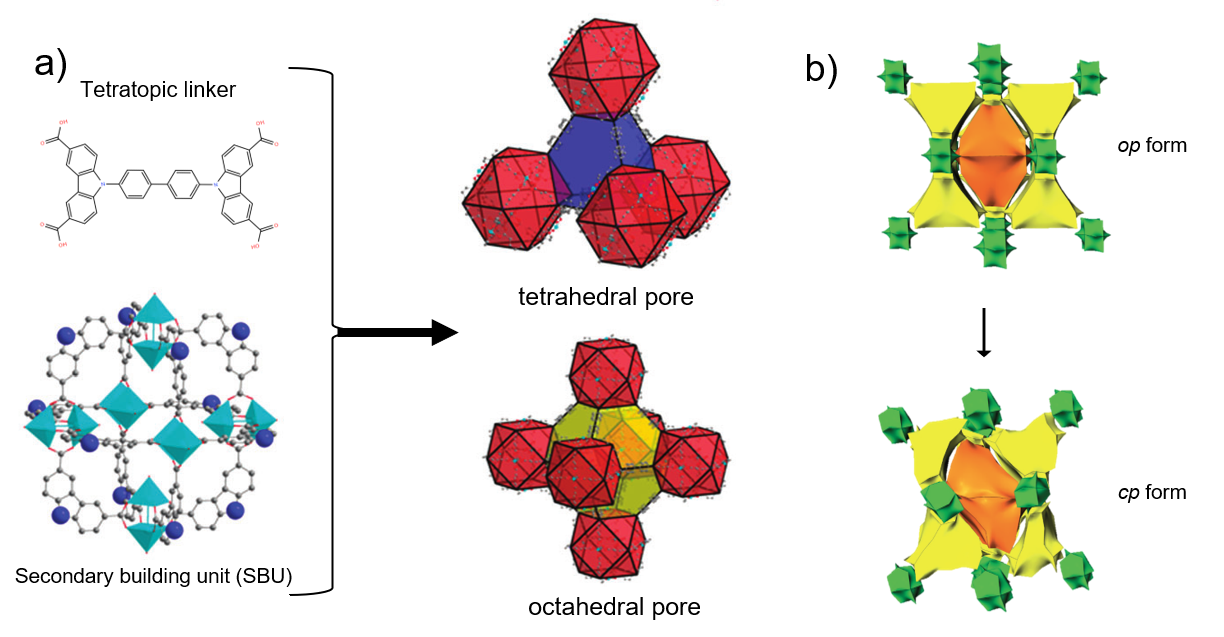
\includegraphics[width=0.9\linewidth]{dut-material}%
    \caption{(a) The tetratopic linker and secondary copper 
    paddlewheel building unit used to synthesise DUT-49, 
    and the resulting structure and generated 
    pores~\cite{stoeckHighlyPorousMetal2012}. (b)
    Two possible phases of the material, with the 
    open to closed pore 
    transition~\cite{krausePressureamplifyingFrameworkMaterial2016}.}%
    \label{dut:fgr:dut-material}
\end{figure}

In the original study, the MOF did not show any flexible behaviour.
However, it was later found by 
\citet{krausePressureamplifyingFrameworkMaterial2016} that 
when adsorbing \ce{CH4} at \SI{111}{\kelvin}, a sharp step occurs
in the isotherm, corresponding to an \textit{op}/\textit{cp} transition. 
More interestingly, the step is accompanied by an expulsion of the
adsorbed gas from the interior of the pores, increasing the pressure
in the experiment cell. This type of pressure-amplifying transition
has been coined negative gas adsorption (NGA) and was found to 
occur with other adsorbates at different temperatures such as \ce{C4H10} 
at \SI{303}{\kelvin} or \ce{Xe} at \SI{195}{\kelvin}, which allowed
study of the transition at ambient temperature and through 
\ce{^{129}Xe} NMR spectroscopy~\cite{schaberSituMonitoringUnique2017}.

The origin of this phenomenon has been elucidated by 
\citet{evansOriginsNegativeGas2016} where it has been shown to 
emerge due to a buckling of the central strut of the 
tetratopic linker under compressive stress induced by adsorption,
similar to the failure of a metal column under critical load.
The \textit{op} and \textit{cp} phase stability depends on the 
adsorbate loading of the material, with the \textit{op} form
being energetically favoured at zero and high loadings. 
At intermediate pore filling, the \textit{cp} state is
stabilized by the fluid molecules and becomes energetically
favoured. At this point, the \textit{op} phase enters
a metastable regime and can contract if the energy barrier between the 
two states is overcome. As the transition from the \textit{cp} to the 
\textit{op} state requires an activation energy, re-opening of the 
structure is only possible through complete structure loading.
If the system is in its \textit{cp} state during adsorbate 
removal, the structure undergoes complete structural collapse.

However, questions still remain about the driving forces
behind the transition itself, such as the contribution of 
guest-host interactions, as well as the temperature range 
and adsorbates where it is possible. The rational design 
of such materials is also put into question, where framework
parameters such as linker length, functionalisation and 
composition may be used to tune the pressure and extent of
NGA. It is here where the adsorption methodology introduced
in \autoref{pyg} combined with \textit{in-situ} calorimetry
as presented in \autoref{calo} can be used to shed light 
on the energetic background of NGA in DUT-49.